\section{Resultados}

\subsection{Número de ejecuciones y validación}

Para la ejecución de nuestros algoritmos separaremos los conjuntos de datos en dos partes, una de entrenamiento y otra de test, utilizando un $80\%$ del conjunto para el entrenamiento y el $20\%$ restante para el test.

De cara a obtener resultados fiables utilizaremos validación cruzada al entrenar, utilizando el método de 5x2 iteraciones, es decir, haremos dos experimentos, cada uno con 5 iteraciones de validación cruzada, y a partir de estos resultados obtendremos el error cuadrático medio resultante.

También tenemos que tener en cuenta que los algoritmos implementados son algoritmos estocásticos, es decir, la aleatoriedad juega una parte importante en las zonas del espacio de soluciones que se explorarán, por este motivo se han realizado cinco ejecuciones distintas, con cinco semillas aleatorias distintas.

\subsection{Parámetros utilizados}

Como vimos en el estado del arte, la Programación Genética es un algoritmo que necesita una población con un gran número de individuos, por este motivo se ha escogido una población de mil individuos. De cara a limitar el sobreajuste de las expresiones y mantener el resultado simple se ha limitado el tamaño máximo de las expresiones a diez nodos.

Con respecto a los demás parámetros se han utilizado los más comunes en otras implementaciones de Programación Genética y que de forma empírica han funcionado mejor en nuestro conjunto de datos.

Se han utilizado los siguientes parámetros:

\begin{itemize}
	\item Tamaño de población: $1.000$.
	\item Probabilidad de que un nodo sea una variable: $30\%$.
	\item Tamaño máximo del árbol: $10$.
	\item Número de evaluaciones: $1.000.000$.
	\item Probabilidad de cruce en PG: $75\%$.
	\item Probabilidad de cruce en GA (solo para GA-P): $75\%$.
	\item Probabilidad de mutación en PG: $5\%$.
	\item Probabilidad de mutación en GA (solo para GA-P): $5\%$.
	\item Probabilidad de cruce intra-nicho (solo para GA-P): $40\%$.
	\item Tamaño del torneo: $100$.
\end{itemize}

\newpage

\subsection{Resultados de Programación Genética}

Tras las distintas ejecuciones con las semillas aleatorias y en cada uno de los conjuntos de datos, obtenemos los siguientes resultados.


\subsubsection{Resultados en la lateralidad izquierda}


\begin{table}[H]
\centering
% \resizebox{\textwidth}{!}{%
\begin{tabular}{|c|c|c|}
\hline
\multicolumn{3}{|c|}{\textbf{Ejecuciones de Programación Genética en la lateralidad izquierda}}                                                \\ \hline
\textbf{Semilla} & \textbf{ECM con 5x2-cv} & \textbf{Expresión obtenida}                                           \\ \hline
12345            & 118,629                 & $( -2.795300  * ( ( x_0  - ( x_0  *  2.079655 ) ) +  4.778957 ) )$        \\ \hline
92034            & 113,681                 & $( x_0  * ( ( 2.955791  /  x_0 ) * ( -4.162967  +  x_0 ) ) )$              \\ \hline
8324             & 116,483                 & $( ( -1.432396  -  7.975771 ) - ( 3.960089  / ( -1.432396  /  x_0 ) ) )$ \\ \hline
34679            & 116,616                 & $( -9.075032  - ( -2.749338  * ( ( x_0  /  x_0 ) *  x_0 ) ) )$             \\ \hline
34634            & 116,644                 & $( ( x_0  + ( -5.473511  / ( x_0  -  9.989626 ) ) ) *  2.327900 )$        \\ \hline
\textbf{Media}   & \textbf{116,4106}       &                                                                       \\ \hline
\end{tabular}%
% }
\caption{Resultados de Programación Genética en la lateralidad izquierda con cinco semillas distintas.}\label{table:resultados_PG_l0}

\end{table}

\subsubsection{Resultados en la lateralidad derecha}


\begin{table}[H]
\centering
% \resizebox{\textwidth}{!}{%
\begin{tabular}{|c|c|c|}
\hline
\multicolumn{3}{|c|}{\textbf{Ejecuciones de Programación Genética en la lateralidad derecha}}                                              \\ \hline
\textbf{Semilla} & \textbf{ECM con 5x2-cv} & \textbf{Expresión obtenida}                                         \\ \hline
12345            & 107,154                 & $( ( x_0  /  6.053368 ) * ( 6.051508  - ( x_0  /  -2.234684 ) ) )$      \\ \hline
92034            & 103,496                 & $( ( 4.069355  * ( -6.973380  +  x_0 ) ) -  1.133718 )$                \\ \hline
8324             & 103,209                 & $( 3.925351  * ( ( 3.575640  - ( 4.634127  -  x_0 ) ) -  5.821175 ) )$ \\ \hline
34679            & 106,156                 & $( x_0  + ( -3.565364  * ( 6.913891  - ( x_0  /  1.292461 ) ) ) )$      \\ \hline
34634            & 107,11                  & $( x_0  * ( ( x_0  + ( 8.715935  /  3.905992 ) ) /  8.165300 ) )$       \\ \hline
\textbf{Media}   & \textbf{105,425}        &                                                                     \\ \hline
\end{tabular}%
% }
\caption{Resultados de Programación Genética en la lateralidad derecha con cinco semillas distintas.}\label{table:resultados_PG_l1}
\end{table}


\subsubsection{Resultados en el conjunto completo}



\begin{table}[H]
\centering
% \resizebox{\textwidth}{!}{%
\begin{tabular}{|c|c|c|}
\hline
\multicolumn{3}{|c|}{\textbf{Ejecuciones de Programación Genética en el conjunto completo}}                         \\ \hline
\textbf{Semilla} & \textbf{ECM con 5x2-cv} & \textbf{Expresión obtenida}                                            \\ \hline
12345            & 112,162                 & $( ( -3.556759  - ( -3.164731  *  x_0 ) ) + ( -5.675591  -  6.310600 ) )$ \\ \hline
92034            & 111,47                  & $( x_0  + ( ( x_0  - ( 3.431506  -  x_0 ) ) -  9.472036 ) )$                \\ \hline
8324             & 111,505                 & $( ( ( ( 2.695238  *  x_0 ) +  -9.196454 ) +  -6.145053 ) /  0.783998 )$  \\ \hline
34679            & 112,22                  & $( 5.258742  * ( ( 5.394186  -  x_0 ) *  -0.634723 ) )$                   \\ \hline
34634            & 109,894                 & $( -3.418017  * ( x_0  - ( ( x_0  -  5.692729 ) +  x_0 ) ) )$               \\ \hline
\textbf{Media}   & \textbf{111,4502}       &                                                                        \\ \hline
\end{tabular}%
% }
\caption{Resultados de Programación Genética en el conjunto de datos completo con cinco semillas distintas.}\label{table:resultados_PG_c}

\end{table}

Como esperábamos, en la mayoría de expresiones podemos ver términos que se podrían reducir, haciendo más simples las expresiones.

Comparando las tablas \ref{table:resultados_PG_l0} y \ref{table:resultados_PG_l1} podemos observar que los resultados son mejores utilizando los datos de la lateralidad derecha, aunque tampoco mejora en exceso el resultado.

Tras estos resultados podemos ver que Programación Genética no obtiene unos buenos resultados, para verlo de una forma más clara tenemos la figura \ref{fig:predicciones_completo_gp}, donde podemos ver con una cruz azul los valores reales del conjunto de test y con una cruz roja la estimación del modelo entrenado con el conjunto de datos completo:

\begin{figure}[H]
	 \centering
	 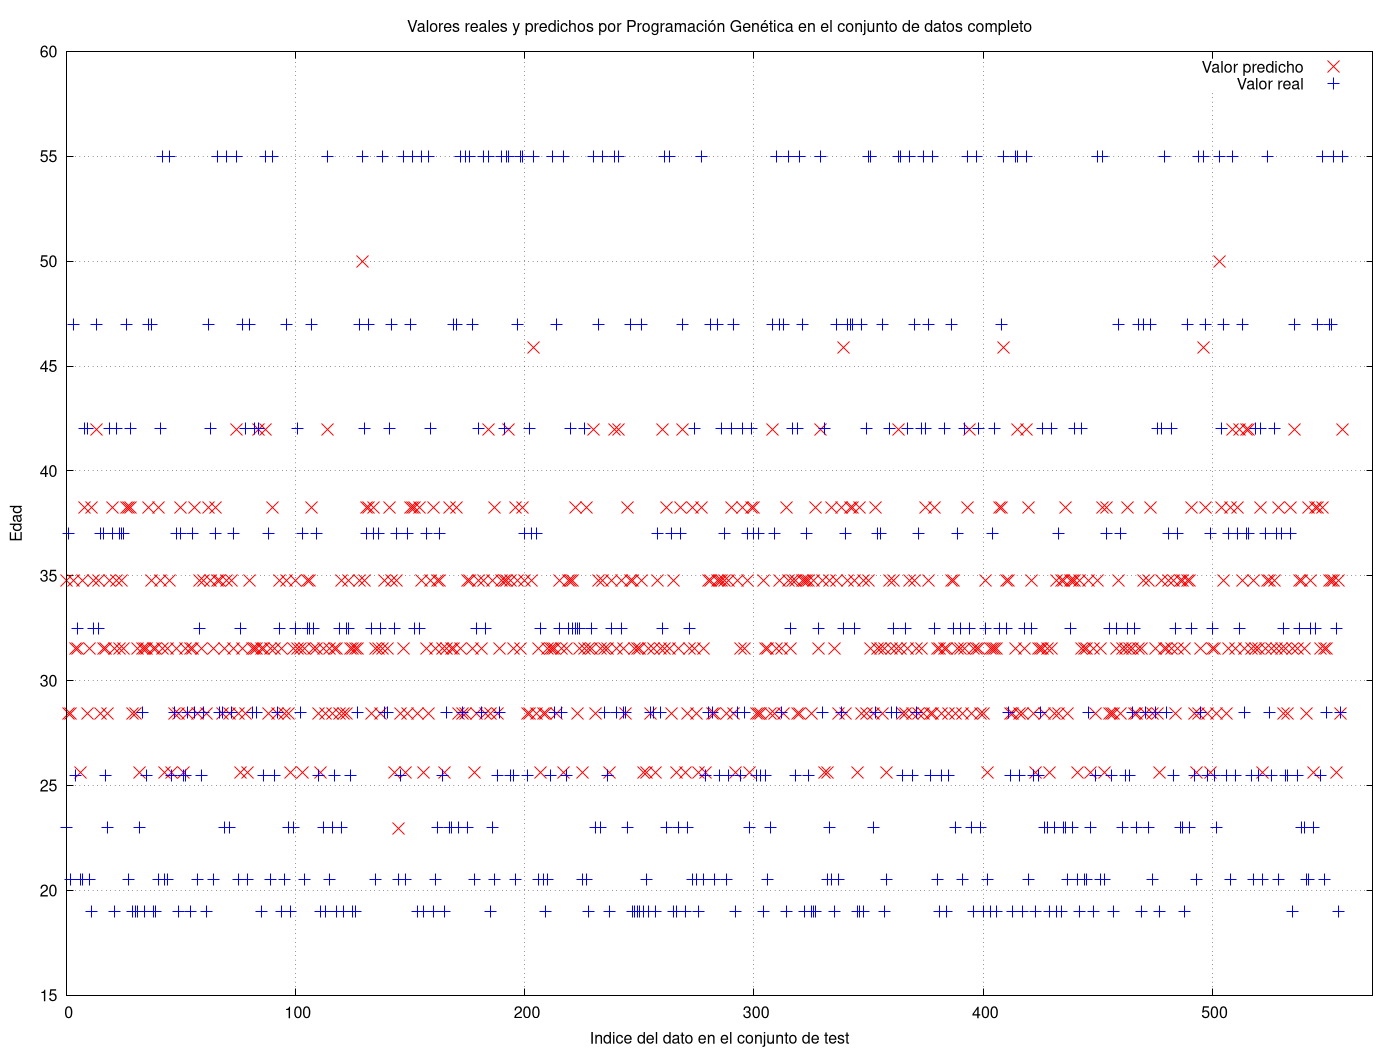
\includegraphics[width=\textwidth]{predicciones_completo_gp.png}
	 \caption{Predicciones de Programación Genética en el conjunto de datos completo.}
	\label{fig:predicciones_completo_gp}
\end{figure}


Vemos como, en general, se suele centrar en las clases intermedias, de entre treinta y cuarenta años, y es que en realidad si el modelo no está seguro de si el valor a predecir es mayor o menor penaliza menos estar en una zona centrada que en el otro extremo de los posibles valores, por lo que asigna un valor intermedio.


\subsection{Resultados de GA-P}

\subsubsection{Resultados en la lateralidad izquierda}


\begin{table}[H]
\centering
% \resizebox{\textwidth}{!}{%
\begin{tabular}{|c|c|c|}
\hline
\multicolumn{3}{|c|}{\textbf{Ejecuciones de GA-P en la lateralidad izquierda}}                         \\ \hline
\textbf{Semilla} & \textbf{ECM con 5x2-cv} & \textbf{Expresión obtenida}                             \\ \hline
12345            & 120,281                 & $( ( x_0  -  -1.232599 ) + ( x_0  -  -1.232599 ) )$         \\ \hline
92034            & 114,659                 & $( x_0  + ( x_0  +  2.316669  ) )$                          \\ \hline
8324             & 118,272                 & $( -3.006461  - ( ( -3.006461  +  x_0 ) *  -3.006461 ) )$  \\ \hline
34679            & 117,77                  & $( x_0  + ( x_0  +  0.855270 ) )$                           \\ \hline
34634            & 119                     & $( ( x_0  +  x_0 ) + ( 5.793486  / ( x_0  -  5.793486 ) ) )$ \\ \hline
\textbf{Media}   & \textbf{117,921}        &                                                         \\ \hline
\end{tabular}%
% }
\caption{Resultados de GA-P en la lateralidad izquierda con cinco semillas distintas.}\label{table:resultados_GAP_l0}

\end{table}

\subsubsection{Resultados en la lateralidad derecha}


\begin{table}[H]
\centering
% \resizebox{\textwidth}{!}{%
\begin{tabular}{|c|c|c|}
\hline
\multicolumn{3}{|c|}{\textbf{Ejecuciones de GA-P en la lateralidad derecha}}                                  \\ \hline
\textbf{Semilla} & \textbf{ECM con 5x2-cv} & \textbf{Expresión obtenida}                                      \\ \hline
12345            & 112,25                  & $( ( 2.750558  /  x_0 ) - ( 2.750558  * ( 2.750558  -  x_0 ) ) )$    \\ \hline
92034            & 108,509                 & $( x_0  + ( x_0  +  2.316669  ) )$                                   \\ \hline
8324             & 109,103                 & $( -2.47599 * ( -1.237995  + ( x_0  /  -1.237995 ) ) )$             \\ \hline
34679            & 108,31                  & $( ( -3.390844  -  x_0 ) - ( x_0  *  -3.390844 ) )$                  \\ \hline
34634            & 111,957                 & $( ( x_0  /  -7.179885 ) * ( -7.179885  - ( x_0  +  -7.179885 ) ) )$ \\ \hline
\textbf{Media}   & \textbf{110,0258}       &                                                                  \\ \hline
\end{tabular}%
% }
\caption{Resultados de GA-P en la lateralidad derecha con cinco semillas distintas.}\label{table:resultados_GAP_l1}

\end{table}


\subsubsection{Resultados en el conjunto completo}


\begin{table}[H]
\centering
% \resizebox{\textwidth}{!}{%
\begin{tabular}{|c|c|c|}
\hline
\multicolumn{3}{|c|}{\textbf{Ejecuciones de GA-P en el conjunto completo}}             \\ \hline
\textbf{Semilla} & \textbf{ECM con 5x2-cv} & \textbf{Expresión obtenida}               \\ \hline
12345            & 114,051                 & $( 0.433841 - ( x_0  * -2.15097351559 ) )$   \\ \hline
92034            & 114,683                 & $( ( -2.527384  -  x_0 ) * -1.836229 )$      \\ \hline
8324             & 114,388                 & $( x_0  / 0.45434982724 )$                   \\ \hline
34679            & 114,386                 & $( -9.634510  * ( x_0 * -0.221638947229 ) )$ \\ \hline
34634            & 112,798                 & $( x_0  * 2.15785599997 )$                   \\ \hline
\textbf{Media}   & \textbf{114,0612}       &                                           \\ \hline
\end{tabular}%
% }
\caption{Resultados de GA-P en el conjunto de datos con cinco semillas distintas.}\label{table:resultados_GAP_c}

\end{table}


En este caso observamos como el problema de las expresiones con partes reducibles se ha reducido drásticamente. Como comentamos, GA-P al tener en cuenta las constantes numéricas como parte de su entrenamiento evita el agrandar la expresión para conseguir el valor que necesita.

Al igual que en Programación Genética, comparando las tablas \ref{table:resultados_GAP_l0} y \ref{table:resultados_GAP_l1}, podemos ver que se comporta mejor en el conjunto de la lateralidad derecha que en el la lateralidad izquierda.

Una cosa a destacar es que viendo los resultados, con GA-P se han obtenido peores resultados que con Programación Genética, a pesar de solucionar el problema del aprendizaje de constantes numéricas. Esto tiene una explicación que podemos deducir fácilmente observando las predicciones sobre el conjunto de test.

\begin{figure}[H]
	 \centering
	 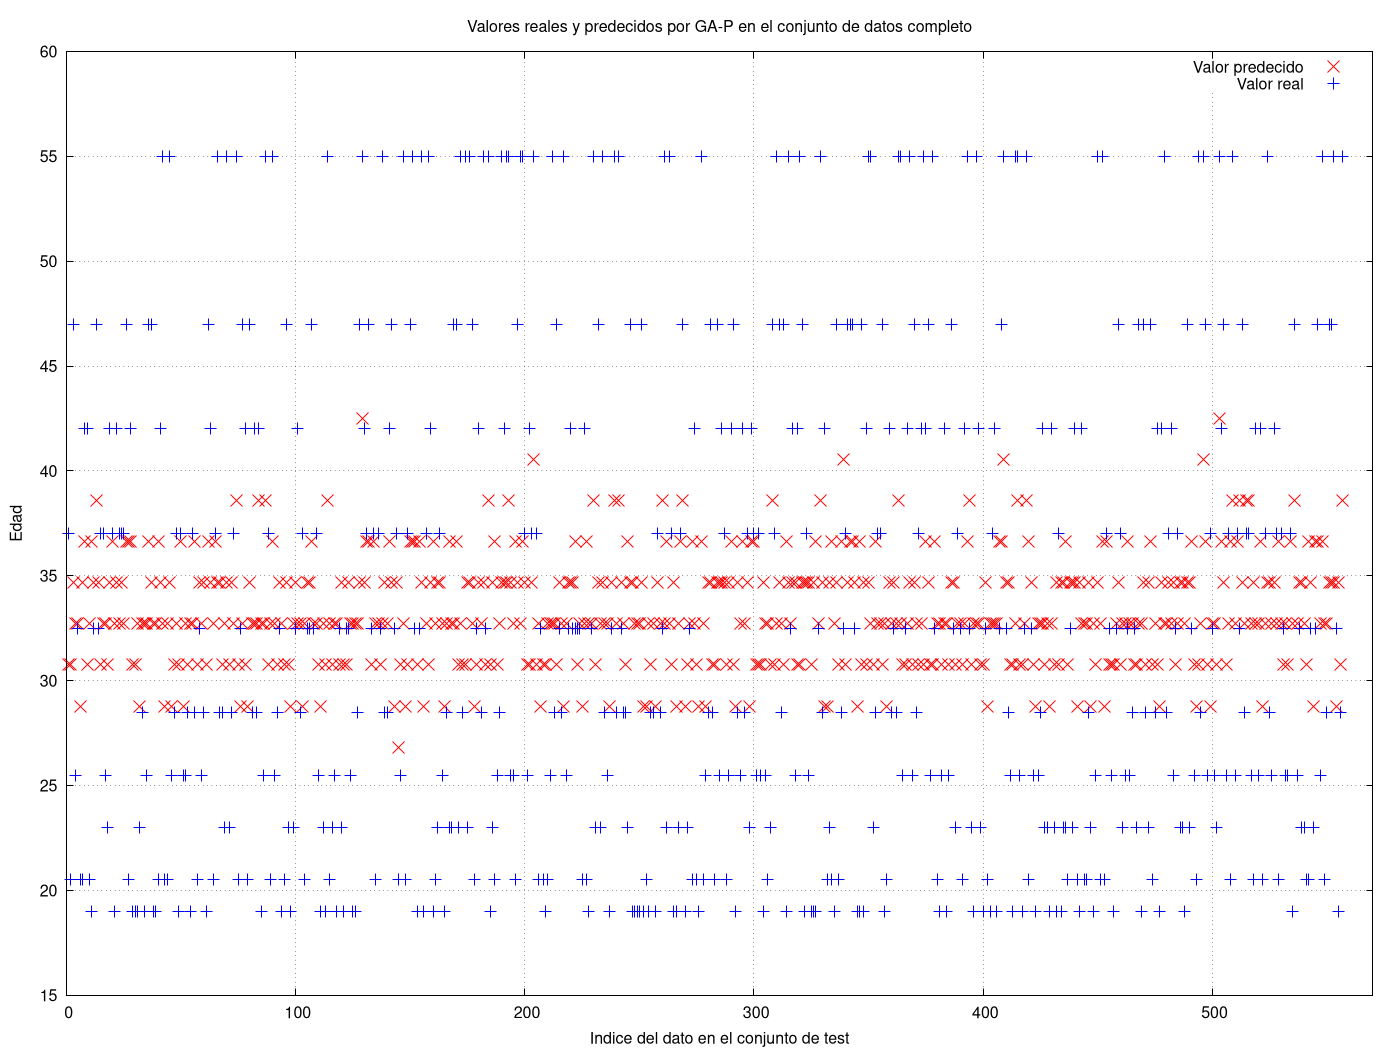
\includegraphics[width=\textwidth]{predicciones_completo_gap.png}
	 \caption{Predicciones de GA-P en el conjunto de datos completo.}
	\label{fig:predicciones_completo_gap}
\end{figure}

Vemos en estas predicciones como en este caso se ha hecho más notable que el algoritmo se centra en valores intermedios, siendo menos de diez predicciones las que se están fuera del rango $[27, 40]$.

De esto podemos deducir que los datos son demasiado similares, y por esto no es capaz de asignar un valor a cada uno de ellos dependiendo de la clase, prefiriendo escoger un valor centrado con respecto a las posibles salidas.


\newpage
